%%%%%%%%%%%%%%%%%%%%%%%%%%%%%%%%%%%%%%%%%%%%%%%%%%%%%%%%%%%%%%%%%%%%%%%%%%%%%%%%%
%																				%
%	TRABAJO:	Trabajo Final													%
%				Especialidad en Ingenier�a en Sistemas de Informaci�n			%
%																				%
%		Titulo:	Procesamiento de Datos en Tiempo Real							%
%																				%
%		Autor:	Juli�n Nonino													%
%																				%
%	Dise�o de la Arquitectura del Sistema										%	
%																				%
%	A�o: 2016																	%
%																				%
%%%%%%%%%%%%%%%%%%%%%%%%%%%%%%%%%%%%%%%%%%%%%%%%%%%%%%%%%%%%%%%%%%%%%%%%%%%%%%%%%

\chapter{Dise�o de la Arquitectura del Sistema}
\label{chapter_arquitectura}

Para cumplir con el objetivo de armar un sistema de procesamiento de dato en
tiempo real utilizando tecnolog�as como Docker, Apache Zookeeper, Apache Kafka y
Apache Storm. Se plantea un sistema multinodo, con cada nodo corriendo un
determinado servicio basado en la imagen de Docker generada.

Como se observa en la figura \ref{arquitectura_general}, se generar�n
tres nodos de Apache Zookeeper, al igual que con Apache Kafka. Esto permite
garantizar la disponibiliad de los servicios. En el caso de Apache Storm, se
generan tres nodos, uno para el procesamiento de datos (podr�an existir m�s), un
�nico nodo encargado de controlar el cl�ster, \emph{Storm Nimbus}, y un nodo
adicional para acceder a la interfaz gr�fica de Apache Storm.

\begin{figure}[H]
	\centering
	\label{arquitectura_general}
	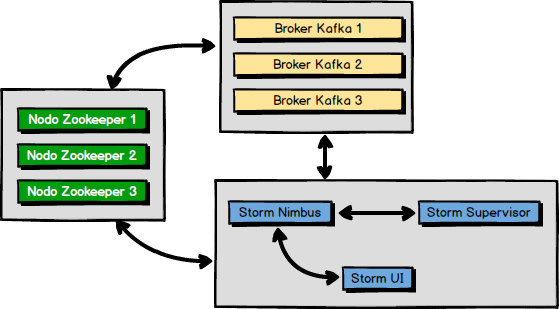
\includegraphics[width=1\linewidth]{./informe/desarrollo/img/ArquitecturaServidor}
	\caption{Arquitectura general del Cl�ster incluyendo Zookeeper, Kafka y Storm}
\end{figure}

\newpage

Tambi�n, se implementan dos simples aplicaciones en Java. Una, para actuar de
productor de datos para Apache Kafka, simulando alg�n dispositivo o sistema que
env�a datos al servidor. La otra es la topolog�a de Apache Storm encargada de
leer los datos desde Apache Kafka y efectuarles alg�n procesamiento. �sta
topolog�a, ser� subida al nodo \emph{Storm Nimbus}.

\begin{figure}[H]
	\centering
	\label{arquitectura_general_clientes}
	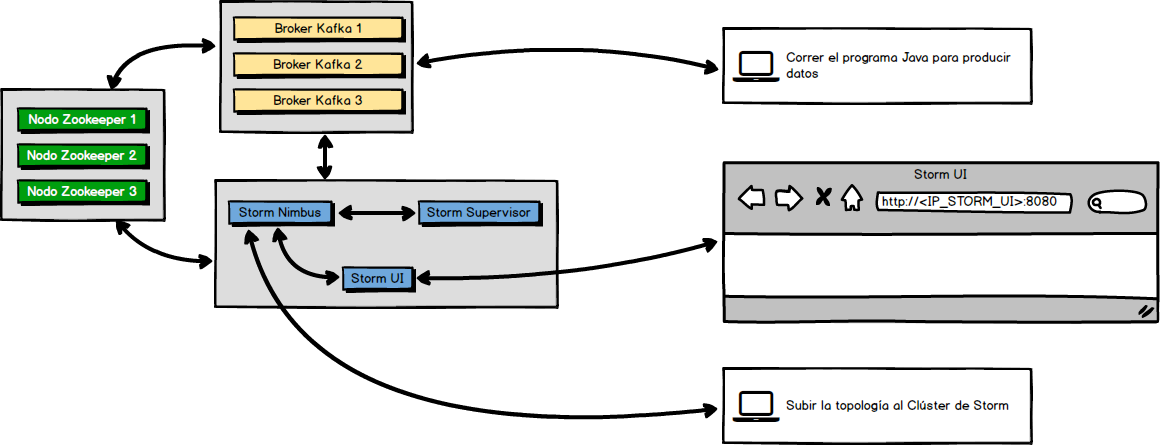
\includegraphics[width=1\linewidth]{./informe/desarrollo/img/ArquitecturaConexionClientes}
	\caption{Arquitectura general del Cl�ster conectado a los programas cliente}
\end{figure}
